%%%%%%%%%%%%%%%%%%%%%%%%%%%%%%%%%%%%%%%%%
% Lachaise Assignment
% LaTeX Template
% Version 1.0 (26/6/2018)
%
% This template originates from:
% http://www.LaTeXTemplates.com
%
% Authors:
% Marion Lachaise & François Févotte
% Vel (vel@LaTeXTemplates.com)
%
% License:
% CC BY-NC-SA 3.0 (http://creativecommons.org/licenses/by-nc-sa/3.0/)
% 
%%%%%%%%%%%%%%%%%%%%%%%%%%%%%%%%%%%%%%%%%

%----------------------------------------------------------------------------------------
%	PACKAGES AND OTHER DOCUMENT CONFIGURATIONS
%----------------------------------------------------------------------------------------
\documentclass{article}

%%%%%%%%%%%%%%%%%%%%%%%%%%%%%%%%%%%%%%%%%
% Lachaise Assignment
% Structure Specification File
% Version 1.0 (26/6/2018)
%
% This template originates from:
% http://www.LaTeXTemplates.com
%
% Authors:
% Marion Lachaise & François Févotte
% Vel (vel@LaTeXTemplates.com)
%
% License:
% CC BY-NC-SA 3.0 (http://creativecommons.org/licenses/by-nc-sa/3.0/)
% 
%%%%%%%%%%%%%%%%%%%%%%%%%%%%%%%%%%%%%%%%%

%----------------------------------------------------------------------------------------
%	PACKAGES AND OTHER DOCUMENT CONFIGURATIONS
%----------------------------------------------------------------------------------------

\usepackage{amsmath,amsfonts,stmaryrd,amssymb} % Math packages

\usepackage{enumerate} % Custom item numbers for enumerations

\usepackage[ruled]{algorithm2e} % Algorithms

\usepackage[framemethod=tikz]{mdframed} % Allows defining custom boxed/framed environments

\usepackage{listings} % File listings, with syntax highlighting
\lstset{
	basicstyle=\ttfamily, % Typeset listings in monospace font
}

%----------------------------------------------------------------------------------------
%	DOCUMENT MARGINS
%----------------------------------------------------------------------------------------

\usepackage{geometry} % Required for adjusting page dimensions and margins

\geometry{
	paper=a4paper, % Paper size, change to letterpaper for US letter size
	top=2.5cm, % Top margin
	bottom=3cm, % Bottom margin
	left=2.5cm, % Left margin
	right=2.5cm, % Right margin
	headheight=14pt, % Header height
	footskip=1.5cm, % Space from the bottom margin to the baseline of the footer
	headsep=1.2cm, % Space from the top margin to the baseline of the header
	%showframe, % Uncomment to show how the type block is set on the page
}

%----------------------------------------------------------------------------------------
%	FONTS
%----------------------------------------------------------------------------------------

\usepackage[utf8]{inputenc} % Required for inputting international characters
\usepackage[T1]{fontenc} % Output font encoding for international characters

\usepackage{XCharter} % Use the XCharter fonts

%----------------------------------------------------------------------------------------
%	COMMAND LINE ENVIRONMENT
%----------------------------------------------------------------------------------------

% Usage:
% \begin{commandline}
%	\begin{verbatim}
%		$ ls
%		
%		Applications	Desktop	...
%	\end{verbatim}
% \end{commandline}

\mdfdefinestyle{commandline}{
	leftmargin=10pt,
	rightmargin=10pt,
	innerleftmargin=15pt,
	middlelinecolor=black!50!white,
	middlelinewidth=2pt,
	frametitlerule=false,
	backgroundcolor=black!5!white,
	frametitle={Command Line},
	frametitlefont={\normalfont\sffamily\color{white}\hspace{-1em}},
	frametitlebackgroundcolor=black!50!white,
	nobreak,
}

% Define a custom environment for command-line snapshots
\newenvironment{commandline}{
	\medskip
	\begin{mdframed}[style=commandline]
}{
	\end{mdframed}
	\medskip
}

%----------------------------------------------------------------------------------------
%	FILE CONTENTS ENVIRONMENT
%----------------------------------------------------------------------------------------

% Usage:
% \begin{file}[optional filename, defaults to "File"]
%	File contents, for example, with a listings environment
% \end{file}

\mdfdefinestyle{file}{
	innertopmargin=1.6\baselineskip,
	innerbottommargin=0.8\baselineskip,
	topline=false, bottomline=false,
	leftline=false, rightline=false,
	leftmargin=2cm,
	rightmargin=2cm,
	singleextra={%
		\draw[fill=black!10!white](P)++(0,-1.2em)rectangle(P-|O);
		\node[anchor=north west]
		at(P-|O){\ttfamily\mdfilename};
		%
		\def\l{3em}
		\draw(O-|P)++(-\l,0)--++(\l,\l)--(P)--(P-|O)--(O)--cycle;
		\draw(O-|P)++(-\l,0)--++(0,\l)--++(\l,0);
	},
	nobreak,
}

% Define a custom environment for file contents
\newenvironment{file}[1][File]{ % Set the default filename to "File"
	\medskip
	\newcommand{\mdfilename}{#1}
	\begin{mdframed}[style=file]
}{
	\end{mdframed}
	\medskip
}

%----------------------------------------------------------------------------------------
%	NUMBERED QUESTIONS ENVIRONMENT
%----------------------------------------------------------------------------------------

% Usage:
% \begin{question}[optional title]
%	Question contents
% \end{question}

\mdfdefinestyle{question}{
	innertopmargin=1.2\baselineskip,
	innerbottommargin=0.8\baselineskip,
	roundcorner=5pt,
	nobreak,
	singleextra={%
		\draw(P-|O)node[xshift=1em,anchor=west,fill=white,draw,rounded corners=5pt]{%
		Question \theQuestion\questionTitle};
	},
}

\newcounter{Question} % Stores the current question number that gets iterated with each new question

% Define a custom environment for numbered questions
\newenvironment{question}[1][\unskip]{
	\bigskip
	\stepcounter{Question}
	\newcommand{\questionTitle}{~#1}
	\begin{mdframed}[style=question]
}{
	\end{mdframed}
	\medskip
}

%----------------------------------------------------------------------------------------
%	WARNING TEXT ENVIRONMENT
%----------------------------------------------------------------------------------------

% Usage:
% \begin{warn}[optional title, defaults to "Warning:"]
%	Contents
% \end{warn}

\mdfdefinestyle{warning}{
	topline=false, bottomline=false,
	leftline=false, rightline=false,
	nobreak,
	singleextra={%
		\draw(P-|O)++(-0.5em,0)node(tmp1){};
		\draw(P-|O)++(0.5em,0)node(tmp2){};
		\fill[black,rotate around={45:(P-|O)}](tmp1)rectangle(tmp2);
		\node at(P-|O){\color{white}\scriptsize\bf !};
		\draw[very thick](P-|O)++(0,-1em)--(O);%--(O-|P);
	}
}

% Define a custom environment for warning text
\newenvironment{warn}[1][Warning:]{ % Set the default warning to "Warning:"
	\medskip
	\begin{mdframed}[style=warning]
		\noindent{\textbf{#1}}
}{
	\end{mdframed}
}

%----------------------------------------------------------------------------------------
%	INFORMATION ENVIRONMENT
%----------------------------------------------------------------------------------------

% Usage:
% \begin{info}[optional title, defaults to "Info:"]
% 	contents
% 	\end{info}

\mdfdefinestyle{info}{%
	topline=false, bottomline=false,
	leftline=false, rightline=false,
	nobreak,
	singleextra={%
		\fill[black](P-|O)circle[radius=0.4em];
		\node at(P-|O){\color{white}\scriptsize\bf i};
		\draw[very thick](P-|O)++(0,-0.8em)--(O);%--(O-|P);
	}
}

% Define a custom environment for information
\newenvironment{info}[1][Info:]{ % Set the default title to "Info:"
	\medskip
	\begin{mdframed}[style=info]
		\noindent{\textbf{#1}}
}{
	\end{mdframed}
}
 % Include the file specifying the document structure and custom commands
\usepackage{lscape}
%----------------------------------------------------------------------------------------
%	ASSIGNMENT INFORMATION
%----------------------------------------------------------------------------------------

\title{Práctica 13} % Title of the assignment

\author{Abel Rosado Peinado - 5265\\ \texttt{abel.rosado@estudiante.uam.es}} % Author name and email address

\date{UAM --- \today} % University, school and/or department name(s) and a date

%----------------------------------------------------------------------------------------

\begin{document}

\maketitle % Print the title
\noindent Queremos encontrar el valor númerico de la siguiente integral elíptica de primera clase 
\[\frac{T}{T'} = \frac{2}{\pi}\int_0^{\frac{\pi}{2}}\frac{d\phi}{\sqrt{1+k^2\sin^2\phi}} \ \ \ \ \ \ k = \sin{\frac{\theta_m}{2}}\]
Que nos da la relación de los periodos de soluciones de las siguientes ecuaciones diferenciales ordinarias respectivamente
\[\ddot{\theta} + \omega_0^2 \sin\theta = 0 \ \ \ \ \ \ddot{\theta} + \omega_0^2 \theta = 0 \]
$\theta_m$ es el valor absoluto del ángulo máximo que se alcanza, y entonces evaluando esa integral para valores desde 0 hasta $5\pi /6$ en intervalos separados por $\pi/36$, obtenemos los valores que se observan en la siguiente figura.

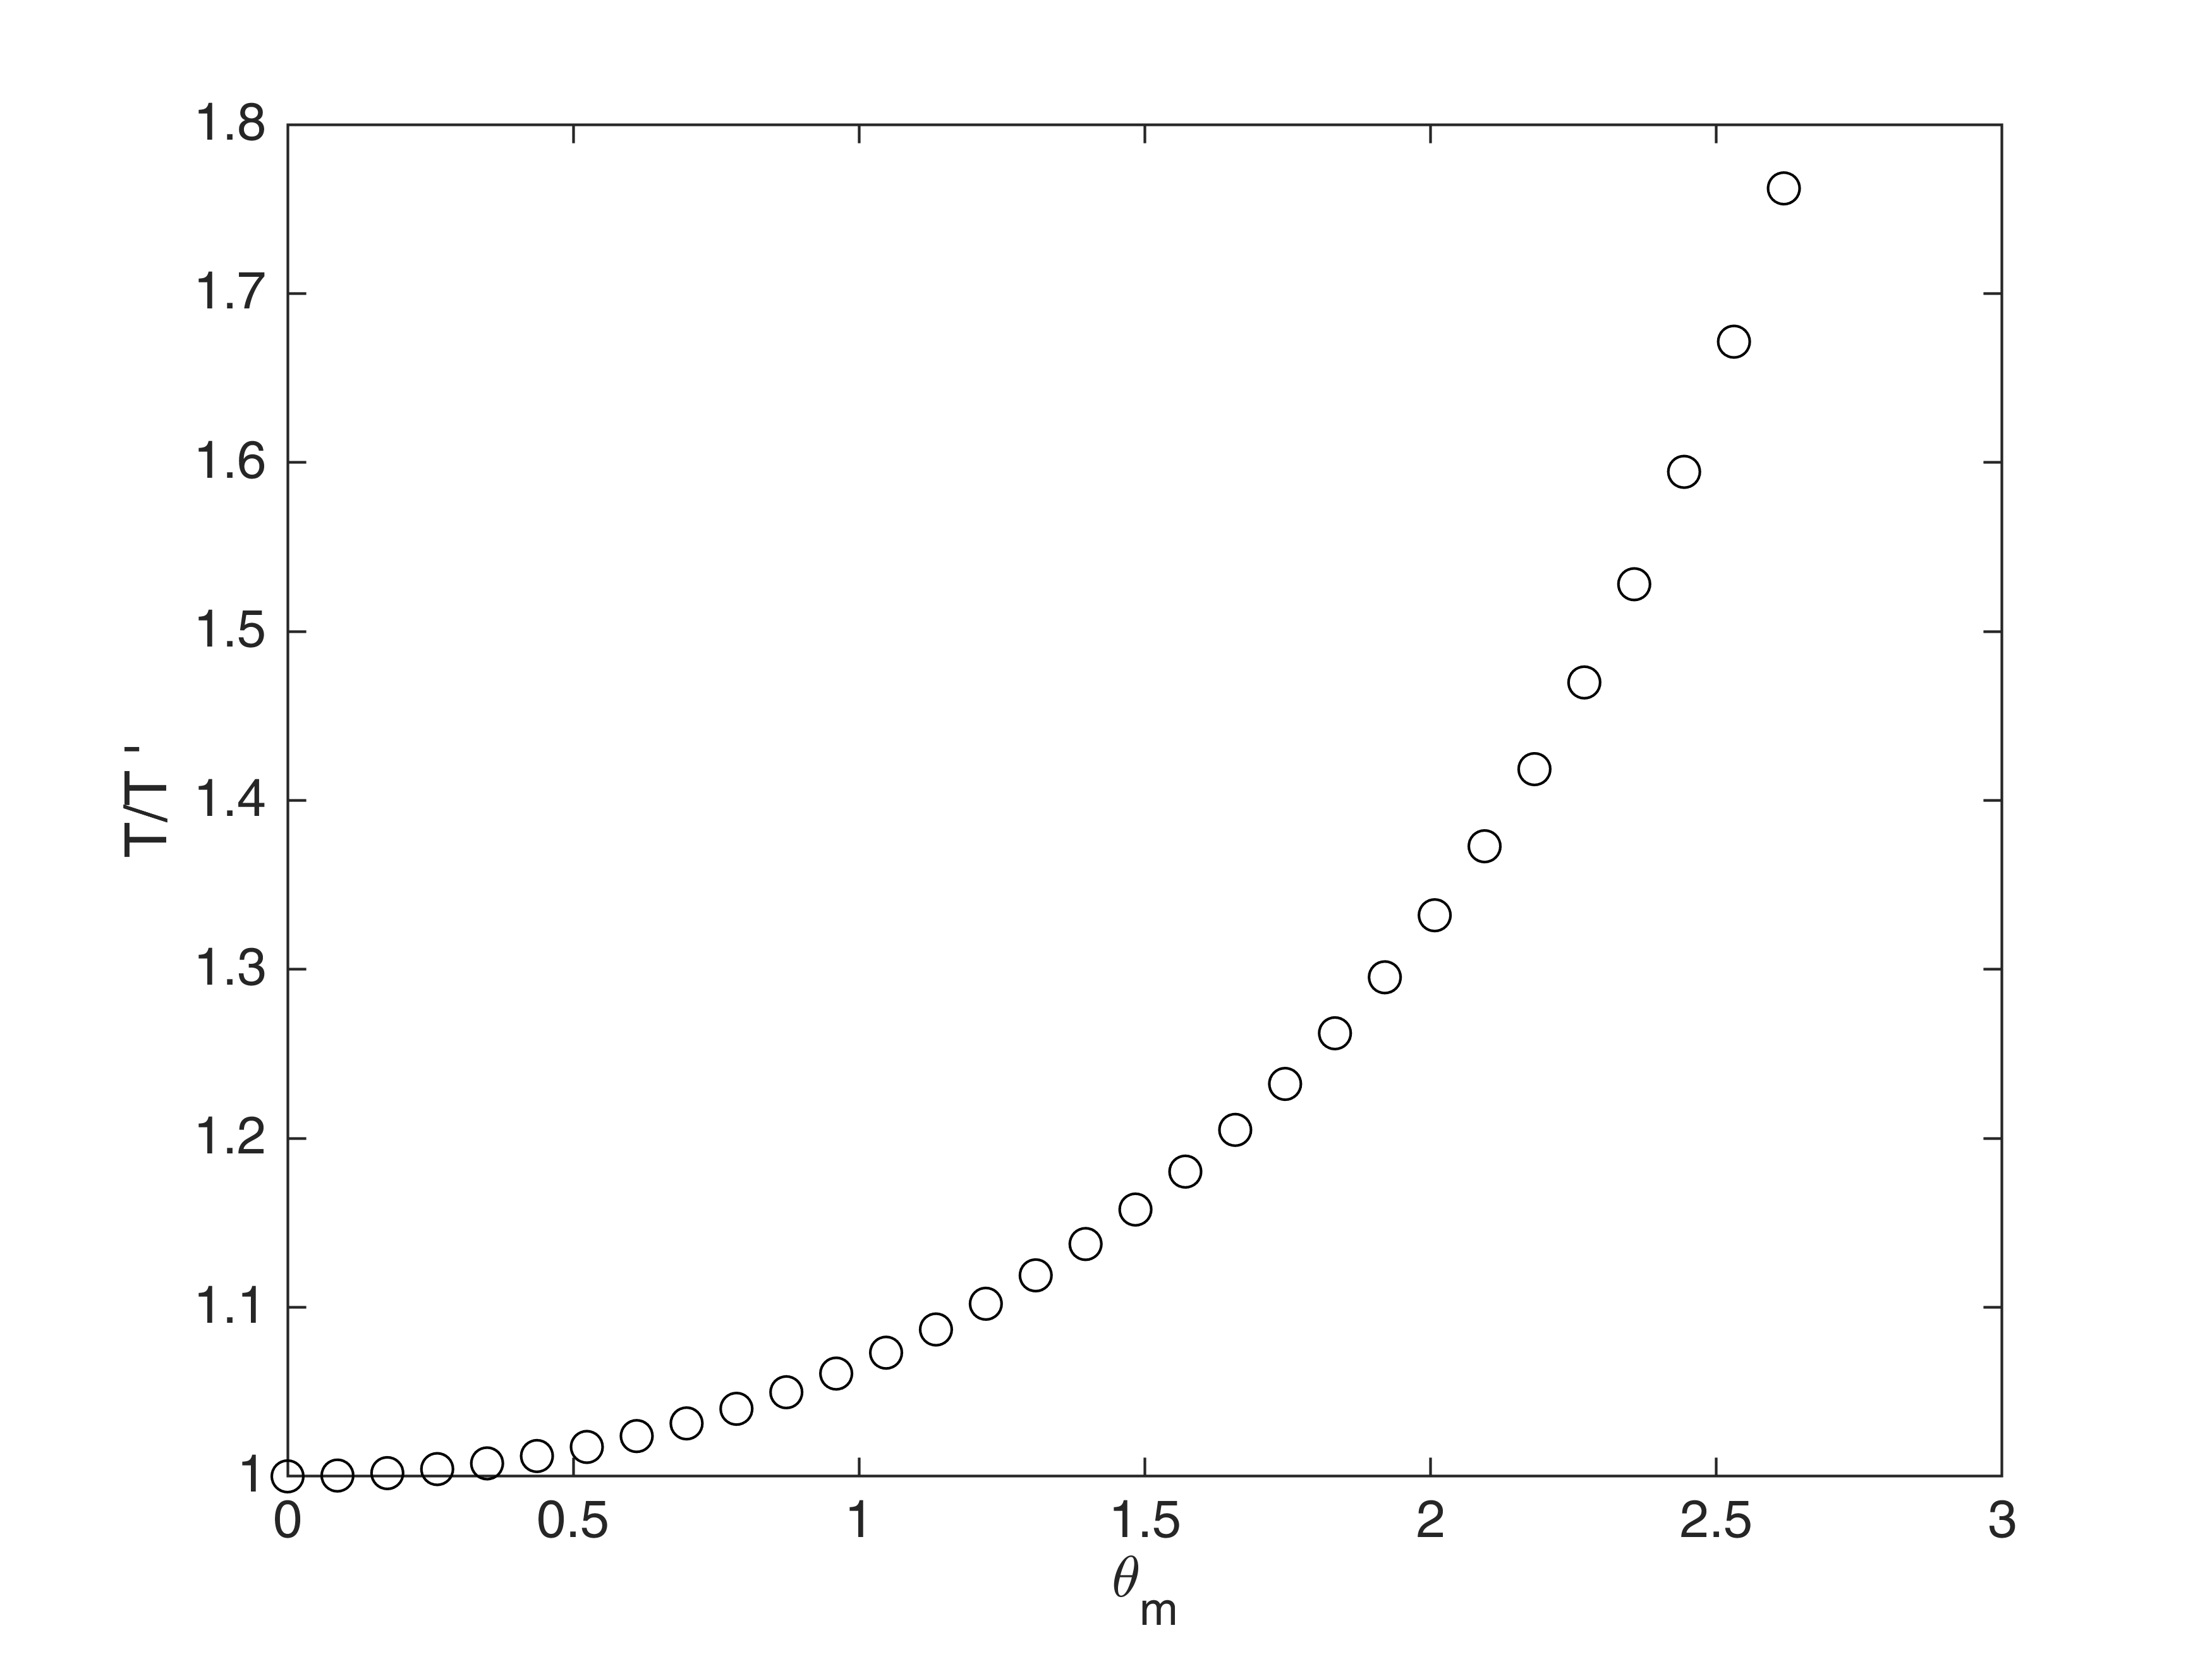
\includegraphics{untitled.png}

Se observa que para el límite $\theta_m \ll 1$, ambos periodos son iguales, lo que esperábamos, puesto que la segunda ecuación es la aproximación de ángulos pequeños de la primera.

La integración se ha realizado utilizando la regla compuesta del trapecio para 4,5 y 20 subintervalos, la regla compuesta de simpson para 4,5 y 20 subintervalos y la cuadratura gaussiana de orden 2 y 5.

\clearpage
\global\pdfpageattr\expandafter{\the\pdfpageattr/Rotate 90}
\begin{landscape}
\begin{table}[]
	\begin{tabular}{|c|c|c|c|c|c|c|c|c|}
	\hline
	\begin{tabular}[c]{@{}c@{}}$\\ \theta_m\\ $\end{tabular} & Trapecio, n=4 & Trapecio, n=5 & Trapecio, n=20 & Simpson, n=4 & Simpson, n=5 & Simpson, n=20 & Gauss, n=2 & Gauss, n=5 \\ \hline
	0                                                        & 1             & 1             & 1              & 1            & 1            & 1             & 1          & 1          \\ \hline
	0.087266463                                              & 1.0004762     & 1.0004762     & 1.0004762      & 1.0004762    & 1.0004764    & 1.0004762     & 1.0004762  & 1.0004762  \\ \hline
	0.17453293                                               & 1.0019072     & 1.0019072     & 1.0019072      & 1.0019072    & 1.0019079    & 1.0019072     & 1.0019078  & 1.0019072  \\ \hline
	0.26179939                                               & 1.0043006     & 1.0043006     & 1.0043006      & 1.0043006    & 1.0043022    & 1.0043006     & 1.0043039  & 1.0043006  \\ \hline
	0.34906585                                               & 1.007669      & 1.007669      & 1.007669       & 1.007669     & 1.0076718    & 1.007669      & 1.0076797  & 1.007669   \\ \hline
	0.43633231                                               & 1.0120306     & 1.0120306     & 1.0120306      & 1.0120305    & 1.0120347    & 1.0120306     & 1.0120568  & 1.0120305  \\ \hline
	0.52359878                                               & 1.0174088     & 1.0174088     & 1.0174088      & 1.0174088    & 1.0174146    & 1.0174088     & 1.0174639  & 1.0174088  \\ \hline
	0.61086524                                               & 1.0238334     & 1.0238334     & 1.0238334      & 1.0238334    & 1.0238408    & 1.0238334     & 1.023937   & 1.0238334  \\ \hline
	0.6981317                                                & 1.0313405     & 1.0313405     & 1.0313405      & 1.0313403    & 1.0313493    & 1.0313405     & 1.03152    & 1.0313405  \\ \hline
	0.78539816                                               & 1.0399733     & 1.0399733     & 1.0399733      & 1.0399729    & 1.039983     & 1.0399733     & 1.040266   & 1.0399733  \\ \hline
	0.87266463                                               & 1.049783      & 1.049783      & 1.049783       & 1.0497818    & 1.0497925    & 1.049783      & 1.0502378  & 1.049783   \\ \hline
	0.95993109                                               & 1.0608292     & 1.0608292     & 1.0608292      & 1.0608268    & 1.0608368    & 1.0608292     & 1.0615094  & 1.0608293  \\ \hline
	1.0471976                                                & 1.073182      & 1.073182      & 1.073182       & 1.0731768    & 1.0731848    & 1.073182      & 1.0741673  & 1.0731821  \\ \hline
	1.134464                                                 & 1.0869225     & 1.0869225     & 1.0869225      & 1.0869121    & 1.0869159    & 1.0869225     & 1.0883124  & 1.0869227  \\ \hline
	1.2217305                                                & 1.1021449     & 1.1021449     & 1.1021449      & 1.1021253    & 1.1021221    & 1.1021449     & 1.1040614  & 1.1021455  \\ \hline
	1.3089969                                                & 1.1189591     & 1.118959      & 1.118959       & 1.118923     & 1.1189099    & 1.118959      & 1.1215498  & 1.1189601  \\ \hline
	1.3962634                                                & 1.1374926     & 1.1374926     & 1.1374926      & 1.1374285    & 1.1374022    & 1.1374926     & 1.1409339  & 1.1374945  \\ \hline
	1.4835299                                                & 1.1578948     & 1.1578947     & 1.1578947      & 1.1577839    & 1.1577415    & 1.1578947     & 1.1623936  & 1.1578978  \\ \hline
	1.5707963                                                & 1.1803409     & 1.1803406     & 1.1803406      & 1.1801534    & 1.1800934    & 1.1803406     & 1.1861358  & 1.1803453  \\ \hline
	1.6580628                                                & 1.2050379     & 1.2050369     & 1.2050369      & 1.2047268    & 1.2046511    & 1.2050369     & 1.2123968  & 1.2050434  \\ \hline
	1.7453293                                                & 1.2322316     & 1.2322293     & 1.2322292      & 1.2317246    & 1.2316409    & 1.2322292     & 1.2414453  & 1.2322371  \\ \hline
	1.8325957                                                & 1.2622178     & 1.2622119     & 1.2622116      & 1.2614031    & 1.26133      & 1.2622116     & 1.2735838  & 1.2622192  \\ \hline
	1.9198622                                                & 1.295355      & 1.295341      & 1.29534        & 1.2940621    & 1.2940353    & 1.29534       & 1.3091484  & 1.2953429  \\ \hline
	2.0071286                                                & 1.3320857     & 1.3320526     & 1.3320497      & 1.3300547    & 1.3301369    & 1.3320497     & 1.3485045  & 1.3320385  \\ \hline
	2.0943951                                                & 1.3729649     & 1.3728889     & 1.3728805      & 1.3698013    & 1.3700953    & 1.3728805     & 1.392036   & 1.3728375  \\ \hline
	2.1816616                                                & 1.4187072     & 1.4185363     & 1.4185126      & 1.4138119    & 1.4144763    & 1.4185126     & 1.4401225  & 1.4184074  \\ \hline
	2.268928                                                 & 1.470262      & 1.4698848     & 1.4698193      & 1.4627227    & 1.4639897    & 1.4698193     & 1.4930986  & 1.4696057  \\ \hline
	2.3561945                                                & 1.5289443     & 1.5281259     & 1.5279476      & 1.5173647    & 1.519551     & 1.5279476     & 1.5511831  & 1.5275668  \\ \hline
	2.443461                                                 & 1.5966749     & 1.5949267     & 1.5944461      & 1.5788973    & 1.5823938    & 1.594446      & 1.6143647  & 1.5938537  \\ \hline
	2.5307274                                                & 1.6764489     & 1.6727656     & 1.6714788      & 1.6490881    & 1.6542927    & 1.6714782     & 1.6822275  & 1.6707342  \\ \hline
	2.6179939                                                & 1.7733147     & 1.7656446     & 1.7622037      & 1.7309275    & 1.7380534    & 1.7621996     & 1.7537054  & 1.7617141  \\ \hline
	\end{tabular}
	\end{table}
\end{landscape}

\end{document}
